\documentclass[a4paper]{article}

\usepackage{hyperref}
\usepackage{geometry}
\usepackage{wasysym}
\usepackage{verbatim}
\usepackage[Q=yes]{examplep} % robust verbatim (eg in description keys)
\usepackage{fancyvrb}
\usepackage{graphicx}
\usepackage[T1]{tipa}
\usepackage{multirow}
%\usepackage{amsmath}
\usepackage{comment} 
\usepackage{rotating}
\usepackage{threeparttable}

%% Package for pretty python code
% \usepackage{minted}

%% Package for pretty code
%\usepackage{listings}
%\usepackage{color}
%\definecolor{mygreen}{rgb}{0,0.6,0}
%\definecolor{mygray}{rgb}{0.5,0.5,0.5}
%\definecolor{mymauve}{rgb}{0.58,0,0.82}
%\lstset{ %
%  backgroundcolor=\color{white},   % choose the background color
%  basicstyle=\footnotesize,        % size of fonts used for the code
%  breaklines=true,                 % automatic line breaking only at whitespace
%  captionpos=b,                    % sets the caption-position to bottom
%  commentstyle=\color{mygreen},    % comment style
%  escapeinside={\%*}{*)},          % if you want to add LaTeX within your code
%  keywordstyle=\color{blue},       % keyword style
%  stringstyle=\color{mymauve},     % string literal style
%}



\title{RUMD Tutorial}
\author{RUMD Development Team}
\hypersetup{
pdftitle={RUMD tutorial},
pdfauthor={RUMD Development Team},
pdfkeywords={Viscous liquids, Molecular dynamics, CUDA}
}

\pagestyle{myheadings}

\hypersetup{pdfborder = {0 0 0}}

\newcommand{\textind}[1]{\mbox{\scriptsize{#1}}}

\newenvironment{example}%
{\bigskip \textbf{\textit{Example}}\\}%
{$\Box$ \newline}

\newenvironment{listing}%
{\verbatim}%
{\endverbatim}

\begin{document}

\maketitle 
\tableofcontents

\newpage

%\documentclass{article}

%\usepackage{geometry}

%\begin{document}

\section{Introduction}
The CUDA project has enabled scientists to utilise NVIDIA's many-core
Graphical Processor Unit (GPU) to solve complex computational
problems. Beside being a very fast processor the GPU is relatively
cheap, and is thus an ideal computational unit for low-cost high
performance supercomputing. Scientific software is currently being
developed in a very rapid pace by many different groups world wide,
and today there exists optimized software for fluid dynamics and
matrix operations just to name a few.   

RUMD [`r\textopeno m di\normalsize$^\bullet$]  
is a high-performance molecular dynamics simulation software package
optimized for NVIDIA's graphics cards. RUMD is designed for small to
medium size systems of spherical particles and simple molecules. RUMD
is developed at The Danish National Research Foundation's centre 
``Glass and Time'' which is located at the Department of Sciences,
Roskilde University.   

\subsection{Features}
RUMD currently supports: 
\begin{itemize}
\item van der Waals type pair potentials: Lennard-Jones, Gaussian
  core, inverse power law, exponential, and more. It is easy to implement new pair
  potentials. 
\item Multicomponent simulations
\item Bond stretching potentials: Harmonic and FENE
\item Bond constraint dynamics
\item Angle bending potentials
\item Dihedral  potentials
\item NVE, NVT, NPT (atomic) and NVU  ensemble simulations
\item Non-equilibrium sheared simulations using Lees-Edwards boundary conditions and the SLLOD equations of motion
\item A Python interface including user-defined on-the-fly analysis.
\item Tools for setting up configuration files, including molecular systems.
\item Post simulation analysis tools
\end{itemize}
In the near future we plan to implement:
\begin{itemize}
\item NPT (molecular) ensemble 
\item Ewald-based Couloumb interactions (a Coulomb potential using direct pair summation and a shifted-force cut-off is available which gives reasonable performance and accuracy for bulk ionic systems)
\end{itemize}

\subsection{User philosophy}
We have defined five users of RUMD:
\begin{enumerate}
\item A user at level 1 is one who can write or copy a simple python script
(for example the one given later in this tutorial) to run a standard molecular 
dynamics simulation, and use the provided analysis tools to perform standard
analysis of the output. This user can make some basic choices, such as the
potential, the integrator, and controlling the frequency of output.
\item This user understands the deeper structure of the code---that is
the different kinds of classes/objects, the relations between them, and their 
interfaces---and understands how the python language works, and can therefore 
write more sophisticated python scripts which
access the full power and flexibility of RUMD.
\item A user at level 3 is one with minimal experience in C++ can write
her own (pair-)potential functions, to be available as classes derived from
\verb|PairPotential|.
\item This user can write their own analysis programs in C++, but does not
need to know anything about GPU programming, since analysis is generally
carried out on the CPU.
\item RUMD developer. Must have a good knowledge of C++, CUDA programming
and knowledge of Subversion.
\end{enumerate}
This tutorial will bring you from level 1 to level 3. Note that level 3 is
higher than level 2 in that it requires the user to write some C++ code and
re-compile the code, but that involves a relatively limited list of things to 
do. Level 2, which stays at the python level, but involves access to almost all of 
the underlying C++ functionality, could take longer to master.


\subsection{Installation}
For Debian-like systems, RUMD can be installed as a package. 
Use the following repository entries appended to 
\textsf{/etc/apt/sources.list} 
or in a file in \textsf{/etc/apt/sources.d/} 
\begin{verbatim}
deb [trusted=yes] http://carid.ruc.dk/rumd buster main
deb-src [trusted=yes] http://carid.ruc.dk/rumd buster main
\end{verbatim}
To install RUMD simply use an equivalent of:
\begin{verbatim}
apt update
apt install rumd rumd-doc python3-rumd
\end{verbatim}
You need to have root privileges, of course. 

You can also build the package from the source. To do so, download the
source code from the RUMD homepage 
\begin{verbatim}
http://rumd.org/download.html
\end{verbatim}
and unpack the file using
\begin{verbatim}
tar xzvf rumd-X.X.tar.xz
\end{verbatim}
where \verb|X.X| is the version number. Enter the source directory 
\begin{verbatim}
cd rumd-X.X
\end{verbatim}
and build the package by typing 
\begin{verbatim}
make
\end{verbatim}
To test your installation use
\begin{verbatim}
make test
\end{verbatim}
This test will take approximately 5-10 minutes.

Notice, you cannot type \verb=make install= since the default path is 
different from system to system. We will refer to the installation
path as \verb=<RUMD-HOME>=  


\subsection{Setting the path for python}

In a proper installation the python  modules should be located in a standard
place where python will automatically find them. This may not be possible if
you do not have root privileges, however. If you have compiled the software
yourself, you need to set the environment variable PYTHONPATH as follows 
For C-shell it would go in your \verb|.cshrc| file; 

\noindent \verb|setenv PYTHONPATH <RUMD-HOME>/Swig:<RUMD-HOME>/Python:<RUMD-HOME>/Tools|

For bash you would add the following to your \verb|.profile|;

\noindent \verb|export PYTHONPATH=<RUMD-HOME>/Swig:<RUMD-HOME>/Python:<RUMD-HOME>/Tools|

\clearpage

%\end{document}

%\documentclass{article}
%\usepackage{verbatim}
%\usepackage{graphicx}
%\usepackage{amssymb,amsmath}
%usepackage{multirow}

\section{Level 1: How to run your first simulation with RUMD }

%\author{LB}
%\date{Level 1}

%\begin{document}
%\maketitle

This tutorial assumes basic GNU/Linux knowledge, a successful
installation of RUMD and a little portion of gumption mixed
with interest in molecular dynamics. For plotting the results 
from simulations it is assumed that xmgrace is installed, but 
other plotting programs can be used if you prefer. 

The basic work-flow of doing simulations is:
\begin{itemize}
  \item Specify initial condition, i.e., the initial positions 
        and velocities to be used in the simulation. This also involves
        the number of particles ($N$) and the (initial) density 
        ($\rho\equiv N/V$).
  \item Running the actual simulation. This can be done interactively 
        or by a script in python. It includes defining how particles 
        interact with each other (i.e., the potentials used), what 
        integrator to use (and the associated parameters, e.g., 
        time-step and temperature.)
  \item Post-processing data analysis.
\end{itemize}
The following sub-sections will take you through these steps.

\subsection{The initial condition}

When conducting simulations it is often convenient to use the end result 
of one simulation as the initial condition to a new simulation.
However, sometimes you need to generate a fresh initial condition. 
This can be done from a terminal window by executing the commands given below. 

First make a directory where you want your first simulation to be performed. Call
it e.g. \verb=~/Test/=, and go to that directory:
\begin{verbatim}
mkdir Test
cd Test
\end{verbatim}
Next, run the \verb=rumd_init_conf= program (make sure  \verb=RUMD_home/Tools/= is 
in your path):
\begin{verbatim}
rumd_init_conf --lattice=fcc --cells=6
\end{verbatim}
This command produces a file called \verb|start.xyz.gz| that we will use as the initial configuration. 
The flag \verb|--lattice=fcc| tells the program to generate a fcc crystal, and 
the flag \verb|--cells=6| that is should make six unit cells in each direction.
The fcc lattice have four particles in the unit cell, and the final configuration
will have $4\times6^3=864$ particles.
%
We have not specified a density or temperature to the program, 
and it will use default values of $\rho=1.0$ and $T=1.0$, respectively. 
Note that \verb|rumd_init_conf| have many options for generating configurations.
A summary of these can be seen by typing
\begin{verbatim} 
rumd_init_conf --help
\end{verbatim}
\verb|rumd_init_conf| also accept ``short arguments'' and the command to generating 
the fcc lattice simply done with
\begin{verbatim}
rumd_init_conf -lfcc -c6
\end{verbatim}

\newlength{\saveparindent}
\setlength{\saveparindent} {\parindent}
\setlength{\parindent}{0 pt}

\subsection{Executing your first program using the python interface}
%
In this first example we will simulate a single component
Lennard--Jones liquid. We will work with python interactively, so that you can
 get a feel for what is possible. For production runs you will normally
make a script containing the appropriate python commands. Start python by typing
\begin{verbatim}
python3
\end{verbatim}
in a terminal. You will get a python prompt that looks like 
``\verb|>>>|''. Type 

\verb|  from rumd import * |

This will import the main RUMD classes into the
global namespace\footnote{Alternatively (recommended by some to avoid possible name clashes in the global namespace) one can type \texttt{import rumd}, and then all of the class-names, etc., must be prefixed by \texttt{rumd.}, for example \texttt{rumd.IntegratorNVE}.} (these are actually C++ classes, but we can ``talk'' to them through python). These are in principle enough to write scripts and thereby run simulations, but to simplify this process, there is an extra python
class called \verb|Simulation|: type
 
\verb|  from rumd.Simulation import Simulation|

This class combines access to the main data-structures 
with the main integration loop and various functions for controlling output 
etc. To start a simulation we first 
create a \verb|Simulation| object, passing the 
name of a starting configuration file:

\verb|  sim = Simulation("start.xyz.gz")|

Here \verb|sim| is an arbitrary name we choose for the object.
Next we choose an NVT integrator, giving the time-step,  temperature and the relaxation time controlling the thermostat [RUMD versions before 3.4 did not require the latter to be explicitly set and set a default value of 0.2]:

\verb|  itg = IntegratorNVT(timeStep=0.0025, targetTemperature=1.0, thermostatRelaxationTime=0.2)|

Having an integrator object, we need to connect it to the simulation:

\verb|  sim.SetIntegrator(itg)|

Next we need to choose the potential. For 12-6 Lennard-Jones we create a 
potential object, giving it the name \verb|pot|, as follows:

\verb|  pot = Pot_LJ_12_6(cutoff_method=ShiftedPotential)|
 
The mandatory argument \verb|cutoff_method| specifies how the cut-off of
the pair-potential is to be handled. It must be one of
\verb|ShiftedPotential| (the most common method, where the potential is
shifted to zero), \verb|ShiftedForce| or \verb|NoShift|
We need to set the parameters, which is done using the method \verb|SetParams|.
The arguments to this method depend on which potential class you are
working with, but they can be found by typing

\verb|  help(pot.SetParams)|

which displays a help page generated from the ``docstring'' of the method
(alternatively type \verb|print pot.SetParams.__doc__|).
In particular this includes a list of the arguments:

\begin{verbatim}
  SetParams(self, unsigned int i, unsigned int j, float Sigma, 
  float Epsilon, float Rcut)
\end{verbatim}


The first one, \verb|self|, represents the object itself, and is not explicitly
given when calling the function. The next two define which particle types we
are specifying parameters for---we just have one type of particle so both will
be zero; the two after that are the standard Lennard-Jones length and energy
parameters, while the last is the cut-off in units of Sigma. Press Q to exit
the help screen. We choose the following:

\verb|  pot.SetParams(0, 0, 1.0, 1.0, 2.5)|

Note that we can also use python's ``keyword arguments'' feature to specify the
arguments, which can then be in any order, for example:

\verb|  pot.SetParams(i=0, j=0, Epsilon=1.0, Rcut= 2.5, Sigma=1.0)|

The potential also needs to be connected to the simulation:

\verb|  sim.AddPotential(pot)|

[The old function \verb|SetPotential| is deprecated as of Version 3.5] Now we are ready to run a simulation. To run a simulation with 20000 time steps,
we just write

\verb|  sim.Run(20000)|

Various messages will be printed to the screen while it is running (these can
 be turned off with \verb|sim.SetVerbose(False)|. If we like, we
can get the positions after the 20000 steps by getting them as a numpy array 
(numpy, or numerical python, is a package that provides efficient array-based
numerical methods), and in particular look at the position of particle 0 by typing

\begin{verbatim}
  pos = sim.sample.GetPositions()
  print pos[0]
\end{verbatim}

However more likely we will run an analysis program on the output
files produced by the simulation during the operation of the \verb|Run|
function. The available analysis programs are described below in subsection~ 
\ref{postProcessing} in their command-line forms. Some of them (eventually all)
can also be called from within python. 
For now let's write a configuration file for possible use as a starting point
for future simulations. Here we go a little deeper into the interface.
Objects of type \verb|Simulation| have an attribute
called "sample" of type Sample 
(the main C++ class representing the sample we are simulating). We call its
\verb|WriteConf| method as follows:

\verb|  sim.WriteConf("end.xyz.gz")|


Type Ctrl-D to exit python. Next we would like to make scripts. Here is the 
script that contains the 
commands we have just worked through (the lines starting with \verb|#|
are comments):


% \begin{lstlisting}[language=python]
% \begin{minted}{python}
\begin{verbatim}
  from rumd import *
  from rumd.Simulation import Simulation

  # create simulation object
  sim = Simulation("start.xyz.gz")

  # create integrator object
  itg = IntegratorNVT(timeStep=0.0025, targetTemperature=1.0, thermostatRelaxationTime=0.2)
  sim.SetIntegrator(itg)

  # create potential object
  pot = Pot_LJ_12_6(cutoff_method=ShiftedPotential)
  pot.SetParams(0, 0, 1.0, 1.0, 2.5)
  sim.AddPotential(pot)

  # run the simulation
  sim.Run(20000)

  # write final configuration
  sim.WriteConf("end.xyz.gz")
\end{verbatim}
% \end{minted}
% \end{lstlisting}


If this script is saved as a file called, for example, run.py (it must end in
.py), then it is run by typing
\verb|python3 run.py|. This will exit python when finished. To leave python on
after the script has completed, type \verb|python3 -i run.py| (-i means run in
interactive mode). If it is to be run on a batch queue, the appropriate PBS
commands should be included in comments at the top as follows:

\begin{verbatim}
  #!/usr/bin/python3
  # pass PYTHONPATH environment variable to the batch process
  #PBS -v PYTHONPATH
  #PBS (other PBS commands here)
  #PBS 
  #PBS 

  # this ensures PBS jobs run in the correct directory
  import os, sys
  if "PBS_O_WORKDIR" in os.environ:
      os.chdir(os.environ["PBS_O_WORKDIR"])
      sys.path.append(".")


  from rumd import *
  (etc)
\end{verbatim}

It should be submitted using \verb|qsub run.py|. Note that the 
indentation of the two lines following the \verb|if| statement is important!

\subsection{Setting options with the python interface}

Here we present some of the options available for controlling simulations.

\subsubsection{Choosing the potential and its parameters}

Probably the most important thing a user needs to control is the 
potential. Different potentials are represented by different classes; objects
are created just as above, so for example:

\begin{verbatim}
  # generalized LJ potential (here m=18, n=4)
  potential = Pot_gLJ_m_n(18,4, cutoff_method=ShiftedPotential) 
  # inverse power-law (IPL) with exponent n=12
  potential = Pot_IPL_12(cutoff_method=ShiftedPotential)
\end{verbatim}


To set parameters for the potential, call its \verb|SetParams| method as 
described above. If a binary system is to be simulated, 
the parameters should be set separately for each interaction pair as follows

\begin{verbatim}
  potential.SetParams(0, 0, 1.00, 1.00, 1.12246)
  potential.SetParams(0, 1, 0.80, 1.50, 1.12246)
  potential.SetParams(1, 1, 0.88, 0.50, 1.12246)
\end{verbatim}

Note that Newton's third law is assumed to hold, so setting the parameters for 
i=0 and j=1 automatically sets those for i=1 and j=0 (we could also have 
called \verb|SetParams| with the latter).
An overview of the available potentials is given in the user manual. 

\subsubsection{Choosing the integrator}

Perhaps the next most important choice is what kind of integration algorithm
to use. Above we did a constant-temperature (NVT) algorithm (the actual
algorithm is of the Nos{\'e}-Hoover type). For constant energy (NVE) runs we
create the integrator as follows, here passing only the time-step:

\verb|itg = IntegratorNVE(timeStep=0.0025)|

(Technical note: this creates an object of the same type as IntegratorNVT,
but here it defaults to NVE mode---in fact in either case one can switch 
thermostatting on or off using the \verb|SetThermostatOn()| method). 

\newlength{\parwidth}
\setlength{\parwidth}{6 cm}


Additional integrators available in RUMD are listed below
\newline \newline
\begin{tabular}{ | l | c | c |}
  \hline  
  \hline
  Name of Integrator & \textbf{Description} & Arguments \\
  \hline
  IntegratorNVE & \parbox{\parwidth}{The \textit{NVE} Leap-frog algorithm.} & \verb=timeStep= \\
  IntegratorNVT & \parbox{\parwidth}{The Nos$\acute{e}$-Hoover \textit{NVT} algorithm.} & \verb=timeStep, targetTemperature, thermostatRelaxationTime= \\
  IntegratorNPTAtomic & \parbox{\parwidth}{\textit{NPT} algorithm. (JCP 101, N 5, 1994)} & \parbox{\parwidth}{ \centering \Q{timeStep, targetTemperature, thermostatRelaxationTime, targetPressure, barostatRelaxationTime} } \\
  IntegratorNVU & \parbox{\parwidth}{Algorithm conserving the total potential energy.} & \verb=dispLength, potentialEnergy= \\
  IntegratorMMC & \parbox{\parwidth}{Metropolis \textit{NVT} Monte Carlo.} & \verb=dispLength, targetTemperature= \\
  IntegratorIHS &\parbox{\parwidth}{ Energy minimization via the Leap-frog algorithm.} & \verb=timeStep= \\
  IntegratorSLLOD & \parbox{\parwidth}{Shear an atomic system in the xy-plane using the SLLOD equations.} & \verb=timeStep, strainRate= \\
  IntegratorMolecularSLLOD & \parbox{\parwidth}{Shear a molecular system in the xy-plane using the SLLOD equations.} & \verb=timeStep, strainRate= \\ 
IntegratorNPTLangevin & \parbox{\parwidth}{Algorithm which generates the \textit{NPT} ensemble using Langevin dynamics} & \verb=timeStep, targetTemperature, friction, targetPressure, barostatFriction, barostatMass= \\
  \hline
  \hline
\end{tabular}
\newline \newline
The above integrators are chosen in the usual way with named arguments as given in the table.
In the case of IntegratorNPTAtomic the user must choose suitable relaxation times for the thermostat and the barostat.
An example of reasonable values for the thermostat and barostat relaxation times for the LJ system at $T=2.0$ and $p=5.0$ are 
\Q{thermostatRelaxationTime=0.4} and \Q{barostatRelaxationTime=10.0}. For IntegratorNPTLangevin the friction may be chosen over a wide range, depending on how strongly individual particles should be coupled to the heat bath. For the box dynamics, note that the ratio of barostatMass to barostatFriction is a relaxation time which should be reasonable for the system (at least long compared to the time step).

\subsubsection{Controlling how frequently to write output}

To control the output written to files we use the \verb|Simulation|
method \verb|SetOutputScheduling|. By default there are two ``output
managers'': ``energies'' and ``trajectory''. The first is for the files 
containing potential/kinetic energies and other global
quantities, while the second is for trajectories (configuration files 
containing the particle positions at different times during the run). 
The write-schedule for either manager
can be evenly-spaced in time (``linear''), 
logarithmic (``logarithmic''), or a  kind of combination of the two 
(``loglin''). Examples of controlling scheduling include

\begin{verbatim}
  sim.SetOutputScheduling( "energies", "linear", interval=50)
  sim.SetOutputScheduling( "energies", "none" )
  sim.SetOutputScheduling( "trajectory", "logarithmic" )
  sim.SetOutputScheduling( "trajectory", "loglin", base=4, maxInterval=64 )
\end{verbatim}

The first causes energies to be output equally spaced (linear) in time, once 
every 50 time steps, while the second turns energy writing off. The third
 will cause logarithmic saving of configurations (where the 
interval between saves doubles 
each time within a ``block'', starting with 1. The fourth does
logarithmic saving starting with interval 4 until the interval 64 is
reached, after which the interval stays fixed at 64 until the end of
the block. The details of log-lin  are described in a separate
document.  By default energies are linear, written every 256 steps,
and trajectories are logarithmic.  


\subsection{\label{postProcessing} Post processing}

The post processing tools are located in the \verb=<RUMD-HOME>/Tools/=
directory and each one of them has a help text. To see the help text
use the option \verb|-h| or \verb|--help| depending on the tool. 
The actual output files generated by the program are in a
directory called \verb|TrajectoryFiles|. When you start a new simulation in the
same directory, this will be moved to \verb|TrajectoryFiles.rumd_bak| as 
a precaution against accidental overwriting of data. The analysis 
programs should be run in the original directory where the simulation was run
(they know they should look in \verb|TrajectoryFiles| for the data).


\verb=rumd_stats= produces mean values, variances and standard
deviations for specific quantities. The \verb=rumd_stats= stdout for
the simulation just performed is shown in table \ref{stat}.  
\begin{table}[!ht]
  \begin{center}
    \begin{tabular}{ l r r r }
      quantity & mean value &  variance & standard deviation \\
      ke     &  1.49802	  &  0.0015541	 &  0.0394221 \\
      pe     & -5.27922	  &  0.0029679	 &  0.0544784 \\
      p	     &  8.64558	  &  0.0529826	 &  0.23018 \\
      T	     &  0.999677  &  0.000692101 &  0.0263078 \\
      Etot   & -3.7812	  &  0.00439295	 &  0.0662794 \\
      W	     &  7.64591	  &  0.052637	 &  0.229428 \\
      \label{stats}
    \end{tabular}
    \caption{rumd\_stats output.}\label{stat}
  \end{center}
\end{table}

Here ke is the kinetic energy, pe is the potential energy, p is the
pressure, T is the kinetic temperature, Ps is the Nose Hoover
thermostat, Etot is the total kinetic energy and W is the virial. The
program writes the mean and variance in the files
\verb=energies_mean.dat= and \verb=energies_var.dat= in one row as the
first column of stdout. 

The radial distribution function is computed by typing 
\verb=rumd_rdf -n 1000 -m 1.0= 
where the first argument is the number of bins in radial
distribution function and the second argument, the minimum time
between successive configurations to use, is to avoid wasting 
time doing calculations that are very similar (we assume here that the
 configurations are  uncorrelated after one time unit). Use
 \verb|rumd_rdf -h| for a full list of arguments. 
The output is \verb=rdf.dat= and for binary systems the columns are:\\
$r \quad g_{00}(r) \quad  g_{01}(r)\quad  g_{10}(r)\quad
g_{11}(r)$. (Single component only has two columns). Plot
\verb=rdf.dat= to obtain figure \ref{rdf}.  
\begin{figure}[!ht]
  \centering
  \includegraphics[scale=0.3]{level1/LJrdf.eps}
  \caption{Radial distribution function.}\label{rdf}
\end{figure}

The static structure factor can be obtained when the radial
distribution function is computed. It is done by typing 
\verb=rumd_sq 2 20 1= 
where the first argument is the start $q$ value, the second
argument is the final $q$ value and the third argument is the
density. The stdout is the $q$ value for the maximum of the first peak
and it is written in a file called \verb=qmax.dat=. The static
structure factor is written in \verb=Sq.dat= and is structured like
\verb=rdf.dat=. Plot \verb=Sq.dat= to obtain figure \ref{LJSq}.\\ 
\begin{figure}[!ht]
\centering
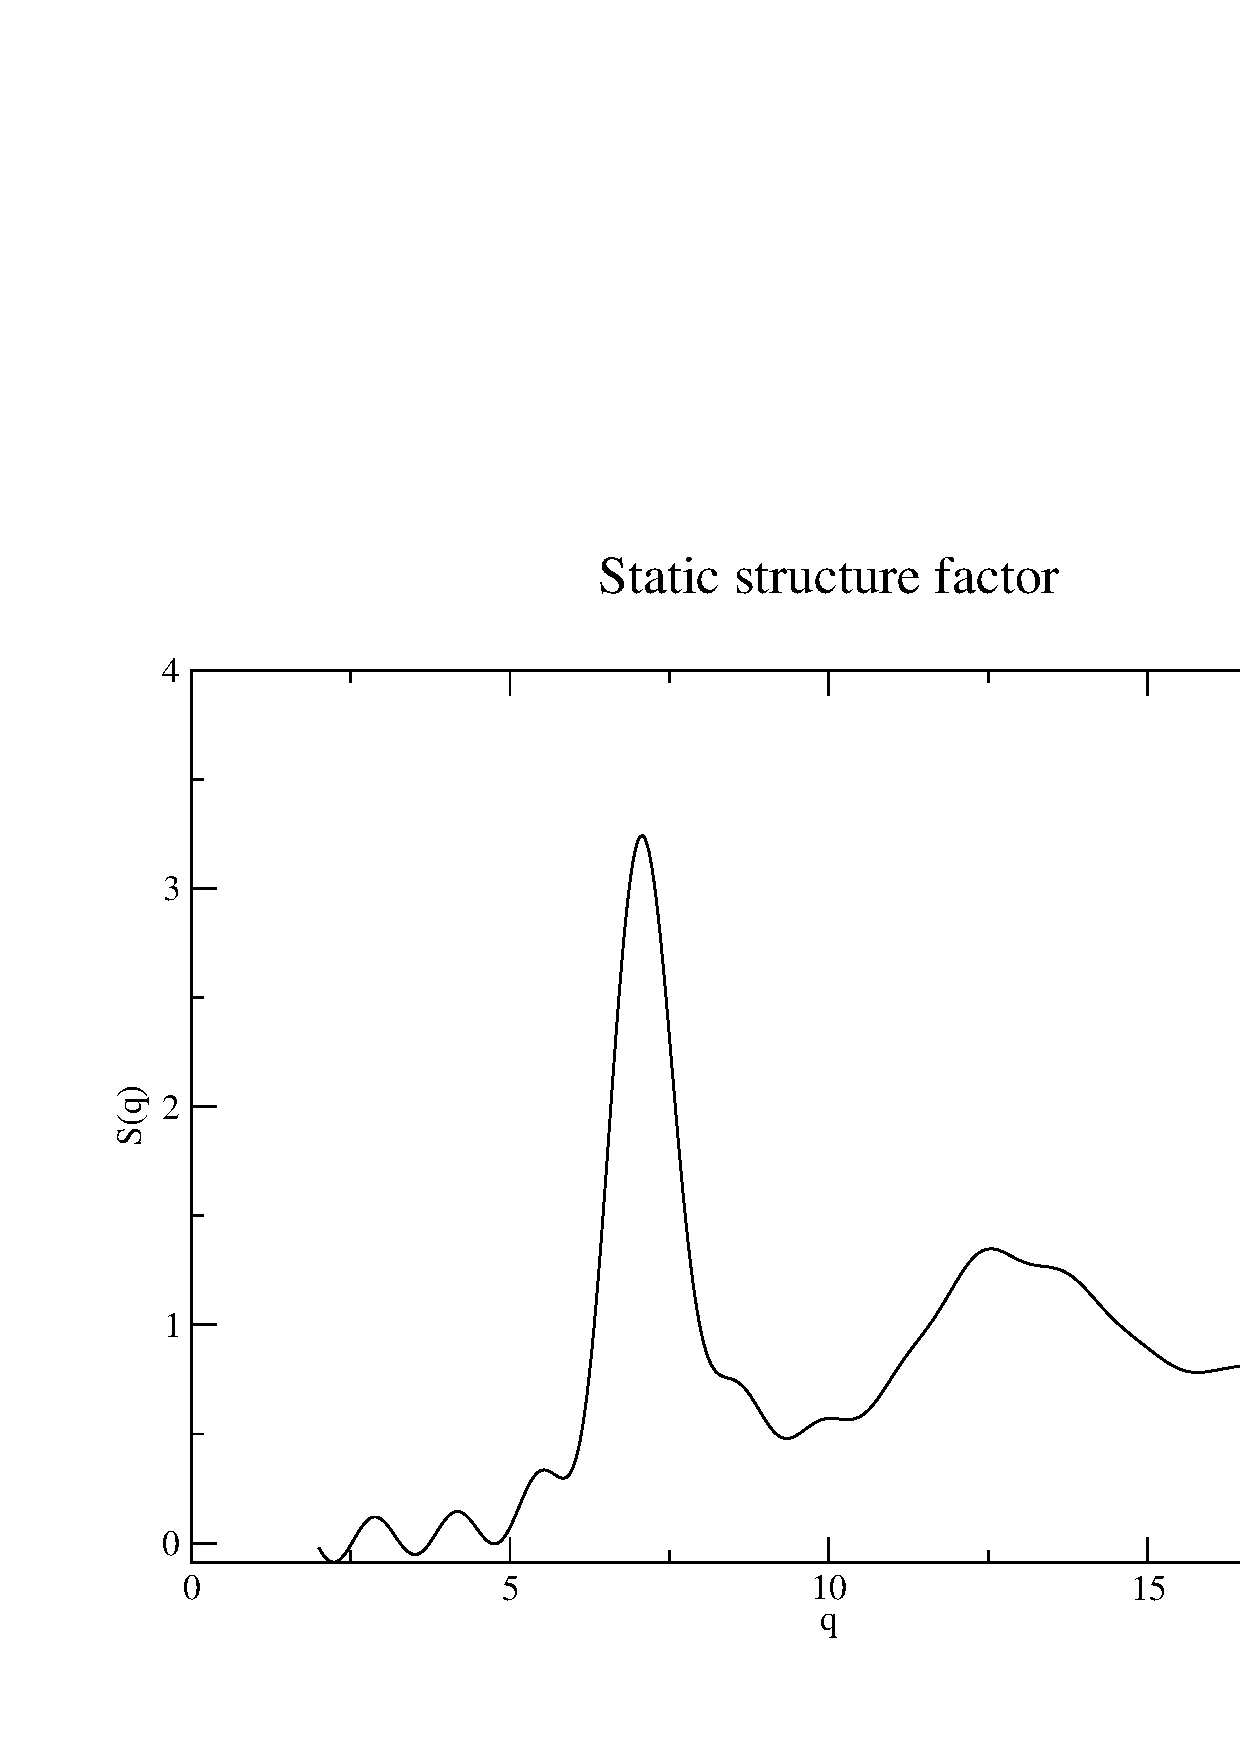
\includegraphics[width=0.6\textwidth]{level1/LJSq}
\caption{The static structure factor}\label{LJSq}
\end{figure}
The mean square displacement and the self part of the
incoherent intermediate scattering function $F_q(t)$ are calculated with 
the command
\verb=rumd_msd=. This generates a \verb=msd.dat= file with time as the
first column and the mean square displacement as a function of time as
the second column (for binary systems there will be two columns), and a file 
\verb|Fs.dat| with a similar structure. Before it can
be run however, you must create a file called \verb|qvalues.dat| which contains
one wavenumber for each type of particle. Typically these correspond to the 
location of the first peak in the structure factor, so one could copy the file
\verb|qmax.dat| created by \verb|rumd_sq|. \verb|rumd_msd| also calculates
gaussian parameter \verb=alpha2.dat=. See figure \ref{msd} and
\ref{Fs} for mean square displacement and self part of incoherent
scattering function.
\begin{figure}[!ht]
\centering
\includegraphics[width=0.6\textwidth]{level1/LJmsd}
\caption{Mean square displacement.}\label{msd}
\end{figure}
\begin{figure}[!ht]
\centering
\includegraphics[width=0.6\textwidth]{level1/LJFs}
\caption{Self part of the intermediate scattering function evaluated
  at the $q$ value of the maximum of the first peak in the structure
  factor.}\label{Fs} 
\end{figure}
The post processing analysis tools are summarized in table \ref{pp}.
 \begin{table}
   \begin{center}
  \begin{tabular}{l c c r}
  \hline \hline
  Tool & Input & Output & Arguments\\
  \hline
  \multirow{3}{*}{rumd\_stats}
   &  & std.out: table \ref{stat} &  \\
   & none & energies\_mean.dat & none \\
   & & energies\_var.dat &  \\
  \hline
  \multirow{3}{*}{rumd\_rdf}
   &  & std.out: Simulation info & 1. num. bins \\
   & none & rdf.dat & 2. time diff. \\
   &  & sdf.dat &  \\
  \hline
  \multirow{3}{*}{rumd\_sq}
   &  & std.out: qmax(s) & 1. qstart \\
   & rdf.dat & Sq.dat & 2. qfinal \\
   &  & qmax.dat & 3. density \\
  \hline
  \multirow{5}{*}{rumd\_msd}
   &  & std.out: Simulation info & \\
   &  & msd.dat  & \\
   & qvalues.dat &  Fs.dat & none\\
   &  &  FsSq.dat & \\
   &  &  alpha2.dat & \\
  \hline \hline
  %\label{pp}
  \end{tabular}
  \caption{Post processing tools, their input, output and the
    arguments.}\label{pp}
\end{center}
 \end{table}
It is evident from table \ref{pp} that \verb=rumd_rdf= has to be
performed before \verb=rumd_sq= and \verb=rumd_sq= before
\verb=rumd_msd=. If you only are interested in the mean square
displacement and know which q-values to use it is not necessary to run
\verb=rumd_rdf= and \verb=rumd_sq= first. Then you just have to create
a file called \verb=qvalues.dat= with the appropriate q-values before
running \verb=rumd_msd=. 



\subsection{Simulating molecules}
With RUMD you can simulate molecular systems. The intra-molecular 
force field includes bond, angle and torsion interactions. The total
potential energy due to intra-molecular interactions excluding
possible pair potentials is given by 
\begin{eqnarray}
\label{eq:intrapot}
U(\vec{r}) = \frac{1}{2}\sum_{\textind{bonds}}k_s^{(i)} (r_{ij}-l_b^{(i)})^2 + 
\frac{1}{2}\sum_{\textind{angles}}k_\theta^{(i)} [\cos(\theta)-\cos(\theta^{(i)})]^2 + 
\sum_{\textind{dihed}} \sum_{n=0}^5 c_n^{(i)} \cos^n(\phi), 
\end{eqnarray}
where $k_s^{(i)}$ is the spring force constant for bond type $i$, $k_\theta^{(i)}$ the 
angle force constant for angle force type $i$, and $c_n^{(i)}$ the torsion 
coefficients for torsional force type $i$. $l_b^{(i)}$ and
$\theta_0^{(i)}$ are the zero force bond length and angle,
respectively. 

Beside the standard harmonic bond potential RUMD also supports
simulation of rigid bonds using constraint method as well as the  
Finite Extensible Nonlinear Elastic (FENE) potential 
\begin{eqnarray}
U(\vec{r}) = -\frac{1}{2}kR_0^2\sum_{\textind{bonds}} \ln\left[ 1 -\left(\frac{r_{ij}}{R_0}\right)^2\right],
\end{eqnarray}
where $k=30$ and $R_0=1.5$ (in reduced units). At the moment 
the constraint method is applicable for molecules with few
constraints.  

\begin{example}
In all one starts by creating (or copying and modifying) a topology file
(with extension \verb|.top|). Examples can be found in the
subdirectory \verb|Conf/Mol|, in particular one called
\verb|mol.top|, which is associated with a configuration file  
\verb|ExampleMol.xyz.gz|. Copy both of these files to your test
directory. They specify a system containing 100 polymeric molecules,
each consisting of  10 monomer units. The appropriate lines to include
in the python script include one for reading the topology file and one
for setting the parameters of the (in this case) single bond-type. Note that this has changed for Version 3.5, so that adding intra-molecular interactions, such as bonds, works similarly to adding ordinary pair interactions.

\begin{listing}
  sim = Simulation("ExampleMol.xyz.gz")
  # read topology file
  sim.ReadMoleculeData("mol.top")

  # create integrator object
  itg = IntegratorNVE(timeStep=0.0025)
  sim.SetIntegrator(itg)

  # create pair potential object
  potential = Pot_LJ_12_6(cutoff_method=ShiftedPotential)
  potential.SetParams(i=0, j=0, Epsilon=1.0, Sigma=1.0, Rcut=2.5)
  sim.AddPotential(potential)

  # define harmonic bond and its parameters for bonds of type 0
  pot_harm = rumd.BondHarmonic()
  pot_harm.SetParams(bond_type=0, bond_length=0.75, stiffness=200.0, exclude=True)
  sim.AddPotential(pot_harm)


  sim.Run(20000)
\end{listing}
Specifying \verb|exclude=True| ensure that contributions from the bonds will be removed from the calculation of the pair potential. If you
wish to keep the pair force interactions between the bonded particles
you can specify this using 

\begin{verbatim}
pot_harm.SetParams(bond_type=0, bond_length=0.75, stiffness=200.0, exclude=False)
\end{verbatim}
\end{example}

If there are other bond-types which have different lengths or stiffnesses, you just call \verb|SetParams| again; it is not necessary to create another \verb|BondHarmonic| object (this will in fact give an error). In the case you wish to use the FENE potential you simply use  
\begin{verbatim}
pot_fene = rumd.BondFENE()
pot_fene.SetParams(bond_type=0, bond_length=0.75, stiffness=30., exclude=False)
sim.AddPotential(pot_fene)
\end{verbatim}
to specify that bond type 0 is a FENE bond type. 
In the FENE potential, the pair interactions between bonded particles
should not be excluded. 

As noted above, you can also simulate molecules with rigid bonds. To 
specify that bond type 0 is a rigid bond you add the bond constraint
using an object of type \verb|ConstraintPotential|:
\begin{verbatim}
pot_cons = rumd.ConstraintPotential()
pot_cons.SetParams(bond_type=0, bond_length=0.75)
sim.AddPotential(pot_cons)
\end{verbatim}

\setlength{\parindent}{\saveparindent}

Details of the format used for the \verb|.top| files and on tools available for
creating them can be found in the user manual.


\clearpage
%\end{document}

%\documentclass{article}
%\usepackage{verbatim}
%\usepackage{graphicx}
%\usepackage{amssymb,amsmath}

\section{Level 2: Fine control} 

%\author{LB}
%\date{Level 2}
%\begin{document}
%\maketitle


The user at level 2 can use the full \verb|Simulation| interface
to control many details of the simulation. Here we 
present, mostly 
in the form of python code-snippets, some of the more advanced 
aspects of the interface, though
without trying to present a complete documentation. The next
step is to look on the RUMD web-page (\verb|rumd.org|) under ``example
scripts'' for ideas about how to get the most out of RUMD.


\subsection{Controlling how the simulation run is divided into blocks}

The simulation output is divided into blocks of size \verb|blockSize|. 
By default the block-size is chosen when \verb|Run| is called, so that
there will be of order 100-200 blocks in the given number of time-steps.
Sometimes it is useful to explicitly specify the block-size (this will sometimes be necessary when using log-lin because there are some constraints on the 
block-size in relation to the log-lin parameters). The following will set
the blockSize (we denote by \verb|sim| the \verb|Simulation| object):

\begin{verbatim}
  sim.SetBlockSize(1024)
\end{verbatim}

\subsection{Controlling what gets written to energies and trajectory files}

To change what gets written we call the \verb|SetOutputMetaData| method, which
functions similar to \verb|SetOutputScheduling| in that it takes a string with 
the name of the output manager, and one or more keyword arguments specifying 
either that a parameter should be included or not, or what the overall 
precision should be.


\begin{verbatim}
  sim.SetOutputMetaData("energies",totalEnergy=False,stress_xy=True, precision=7)
\end{verbatim}
which turns off writing the total energy, turns on writing the xy component
of the stress tensor, and sets the precision to seven decimal places. 
Table~\ref{energyQuantities} shows the most important available
quantities. To each of these are associated two strings: an ``identifier'' for
use in scripts, to refer to a given quantity when turning it ``on'' or ``off'';
and a ``column-label'', which appears in the comment-line of the energies file
to identify which column corresponds to which quantity.

\begin{table}
  \caption{\label{energyQuantities}Identifier and column-label for the main
    quantities that can be written to the energies file.}
  \begin{center}
    \begin{threeparttable}
      \begin{tabular}{|c|c|}
        \hline
        identifier & column label \\
        \hline
        \verb|potentialEnergy| & \verb|pe| \\
        \verb|kineticEnergy| & \verb|ke| \\
        \verb|virial| & \verb|W| \\
        \verb|totalEnergy| & \verb|Etot| \\
        \verb|temperature| & \verb|T| \\
        \verb|pressure| & \verb|p| \\
        \verb|volume| & \verb|V| \\
        \verb|stress_xx| & \verb|sxx| \tnote{(a)} \\
        \hline
      \end{tabular}
      \begin{tablenotes}
      \item[(a)] Potential part of atomic stress. Similarly yy, zz, xy, etc
      \end{tablenotes}
  \end{threeparttable}
  
\end{center}
\end{table}



For simulations in which more than one potential is present, 
the contributions from different terms
to the total potential energy can be included in the energies file. Each 
potential class has an ID string. For example for \verb|Pot_LJ_12_6| it is 
``potLJ''. If desired the ID string can be changed (for example to the simpler 
``LJ'') via

\begin{verbatim}
  pot.SetID_String("LJ")
\end{verbatim}
In the case of contributions to potential energy this ID-string functions as
both the identifier in scripts, and the column-label in the energies-file.
So for example, after changing the ID-string to ``LJ'' as above, to cause it 
to be written we would write

\begin{verbatim}
  sim.SetOutputMetaData("energies", LJ=True)
\end{verbatim}
There is a mechanism for additional quantities to be defined and included in
the energies file, via classes of type \verb|ExternalCalculator|. This is
described in the user manual.

\subsection{Changing the sample volume within the script}

It can be useful to take a configuration corresponding to one density and
rescale the box and particle coordinates such that it has a different density.
This is accomplished by the following lines (which also show how to get the
current volume and number of particles).

\begin{verbatim}
  nParticles = sim.GetNumberOfParticles()
  vol = sim.GetVolume()
  currentDensity = nParticles/vol
  sim.ScaleSystem( pow(newDensity/currentDensity, -1./3) )
\end{verbatim}
where \verb|newDensity| is understood to be the desired density.

\subsection{Options for Run: Restarting a simulation, 
suppressing output, continuing output}

Under default conditions a ``restart file'' will be written, once per 
output-block. If a simulation is interrupted (due to hardware problems for 
example), it can be restarted from the last completed 
block (here 12) by
 
\begin{verbatim}
  sim.Run(20000, restartBlock=12)
\end{verbatim}
where the original number of time-steps should be specified, and the last
completed block can be found by looking at the file 
``LastComplete\_restart.txt'' in TrajectoryFiles. It is possible to suppress 
writing of restart files (so restarts will not be possible), 
and all other output, by calling

\begin{verbatim}
  sim.Run(20000, suppressAllOutput=True)
\end{verbatim}
This might be done for example, during an initial period of equilibration, 
although if this is planned to take a long time, it may be advisable to allow
restart files to be written, in case of possible interruptions.

To avoid re-initializing the output, so that repeated calls to Run will 
append to the existing energies and trajectory files, do

\begin{verbatim}
  sim.Run(20000, initializeOutput=False)
\end{verbatim}
This will give an error if \verb|Run| was not called previously in the normal
way (\verb|initializeOutput=True|, which is its default value).


\subsection{Getting optimum performance via the autotuner}

RUMD involves several internal parameters whose values do not affect the 
results of the simulation within round-off
error, but they can have a noticeable effect on performance. The easiest way
to identify the optimal values is to use the autotuner, which is a python
script that takes a simulation object which is ready to run (the potential(s)
and integrator have been set), and determines the best values for the internal
parameters. The following snippet shows how this is done.

\begin{verbatim}
from rumd.Autotune import Autotune
at = Autotune()
[create sim with associated potential(s) and integrator]
at.Tune(sim)
sim.Run()
\end{verbatim}

The time taken to do the tuning is of order a minute for small systems
(longer if constraints are involved). The autotuner writes a file,
\verb|autotune.dat| in the directory. If the simulation is re-run in the same
directory with the same user parameters and on the same type of graphics card, 
then the autotuner will simply use the previously determined internal 
parameters.

\clearpage

%\end{document}

%\documentclass{article}
%\usepackage{amssymb,amsmath}
%\usepackage{comment} 
%\usepackage{graphicx}
\section{Level 3: How to implement your own pair potential in RUMD}

%\author{LB}
%\date{Level 3}
%\begin{document}
%\maketitle
%\noindent
This tutorial will describe how to implement a new pair potential and
test it. Let us say we want to implement a Gaussian core potential: 
\begin{equation}
v(r) = \epsilon \exp\left[ -\left( \frac{r}{\sigma} \right)^2 \right]
\end{equation}


When implementing a new pair potential there are a number of things to do:
\begin{enumerate}
  \item Implement the potential and force into the RUMD source code
  \item Include the new potential in the Python interface 
  \item Compile
  \item Test the potential
  \item Use it
\end{enumerate}

The \verb|PairPotential.h| in the directory <RUMD-HOME>/include /rumd
contains all the pair potentials, implemented as classes in C++. 

We start with a review of the general 12-6 Lennard-Jones potential - it is 
the first pair potential in the file (search for \verb|Pot_IPL_12_6|). Note
that this is not the one most typically used in simulations; that would be
one of its derived classes \verb|Pot_LJ_12_6|. The difference is only in how
the parameters are specified: for the \verb|Pot_IPL_12_6| potential, rather
than \verb|Epsilon| and \verb|Sigma|, we specify the coefficients of the IPL
terms, \verb|A12| and \verb|A6|. We will 
make a copy of it and change it to the Gaussian core potential. 

The implementation is split into two major parts: The first part is the 
function \verb|SetParams(...)| which is called by the user via the 
python interface. The last part is the function \verb|ComputeInteraction| 
where the actual  computation (on the GPU) is taking place. 


\verb|SetParams(...)| is called via the python interface once for
each type of interaction, with \verb|i| and \verb|j| denoting the types
of the two particles involved in the particular
interaction. The user specifies the coefficients $A_{12}$ and $A_6$
and the cut-off $R_{cut}$ (in other potentials the parameters might include a
characteristic length $\sigma$ and 
characteristic energy $\epsilon$ and possibly more parameters).
The parameters of the potential are communicated by storing them in 
\verb=h_params[i][j][]=.  NOTE: the correctness of the program relies on \verb=h_params[i][j][0]= containing the cut-off in absolute units. 
In other words, interactions between particles of type \verb|i| and \verb|j|
are only computed if the distance between the two particles is less than
 \verb=h_params[i][j][0]=. The rest
of the stored parameters are chosen to facilitate fast computation.

The actual computation of the potential and the associated force 
is done on the GPU by the 
function \verb|ComputeInteraction(...)|. When this is called 
\verb|dist2| contains the square of the distance between the two 
particles in question, and \verb|param| contains the appropriate 
parameters as set up by  \verb| SetParams(...)|. From this information, 
the function calculates  $s$ (i.e. the force, see below in equation
(\ref{s})) and the potential. In the Lennard-Jones
potential it is convenient to define two inverse lengths
\verb|invDist2| and \verb|invDist6| to minimize the number of
calculations. With these
lengths it is easy to calculate $s$ and the potential energy.
\verb|(*my_f).w +=| is the contribution to the potential energy.

We will now proceed to implement a Gaussian core potential. First 
step is to write up the equations we will implement. We will here 
implement the Gaussian core potential (repeated below)
\begin{equation}
   v(r) = \epsilon \exp\left[ -\left( \frac{r}{\sigma} \right)^2 \right]  
\end{equation}

We have to provide the function $s$ which is used 
by RUMD to calculate the force:
\begin{equation}
   s(r) \equiv -\frac{1}{r}\frac{d U(r)}{d r} = \frac{2 \epsilon}{\sigma^2}\exp\left[ -\left( \frac{r}{\sigma} \right)^2 \right] \label{s}
\end{equation}

Now copy the entire Lennard-Jones potential and paste it somewhere in the file
\verb|PairPotential.h|. Replace \verb|Pot_IPL_12_6| with \verb|Pot_Gaussian| 
(four places).
Choose a default identity string, e.g. \verb|SetID_String("potGauss");|.

We will change the arguments in the \verb| SetParams(...)| to match those of
the other LJ potential \verb|Pot_LJ_12_6| which uses $\epsilon$ and $\sigma$ 
instead of $A_{12}$ and $A_6$, since
the Gaussian potential also has a characteristic length $\sigma$ and a 
characteristic energy $\epsilon$. But we need to make corresponding
changes to the \verb|h_params[i][j][]|'s. For the Gaussian potential they
become: 
\begin{itemize}
  \item \verb|h_params[i][j][0] = Rcut * Sigma;|
  \item \verb|h_params[i][j][1] = 1.f / ( Sigma * Sigma );|
  \item \verb|h_params[i][j][2] = Epsilon;|
\end{itemize}
Note that here the user parameter \verb|Rcut| is to be interpreted as a scaled
cutoff, in units of the corresponding $\sigma$.
 Now we can write the part taking place on the GPU. Since we do
not need any inverse distances delete the lines computing 
\verb|invDist2| and \verb|invDist6|. We define instead a 
float called \verb|Dist2|:
\begin{verbatim} 
float Dist2 = dist2 * param[1];
\end{verbatim}
which is $(r/\sigma)^2$. To avoid computing the exponential more than once, we define:
\begin{verbatim} 
float exponential =  exp(-Dist2);
\end{verbatim}
With these definitions, $s$ is simply implemented as:
\begin{verbatim}
float s = 2.f * param[1] * param[2] * exponential;
\end{verbatim}
The next line is the potential:
\begin{verbatim}
(*my_f).w += param[2] * exponential;
\end{verbatim}

This finishes the actual implementation, and we now proceed with a number of more technical changes ensuring that RUMD knows your new pair potential exists. 
\begin{itemize}
  \item In the file \verb|Potentials.i| in the directory 
        <RUMD-HOME>/Swig copy the entry (see below) relating to 
        \verb|Pot_IPL_12_6|, replace \verb|Pot_IPL_12_6| with your potential name, change the arguments to \verb|SetParams| in accordance with how it was defined in \verb|PairPotential.h|, and replace the docstring with a similar brief description of your potential. To be 100\% clear about what needs to be copied, here is the entry for \verb|Pot_IPL_12_6|:

\begin{verbatim}
// docstring for Pot_IPL_12_6
%feature("autodoc","Standard 12-6 Lennard-Jones (cut and shifted potential)
v(r) =  ( A12/r^12  +  A6/r^6 ) - v_cut
s(r) = 12 A12/r^14 + 6 A6/r^8  = -r^-1*dv/dr (F_ij = s * r_ij)") Pot_IPL_12_6;

class Pot_IPL_12_6 : public PairPotential
{
 public:
  Pot_IPL_12_6( CutoffMethod cutoff_method );
  void SetParams(unsigned int i, unsigned int j, float A12, float A6, float Rcut);
};
\end{verbatim}

  \item In the directory <RUMD-HOME> do\\
        \verb|make|        
\end{itemize}


If everything compiled without errors the new pair potential will 
now be available from the python interface, and you need to test 
it. Run a simulation as described in the Level 1 tutorial, but choose the 
new potential.  

Check that the simulation ran with the correct potential by plotting 
it by adding \\ 
\verb|potential.WritePotentials(sim.sample.GetSimulationBox())|
to your script. This command produces a file ''potentials\_\verb=PotID=.dat'' where the potential $v(r)$ is followed by the radial force $f(r)$ in each column for all 
possible particle pairs.

Make sure that the cut-off is done correctly by the program by zooming in on that distance. An example is shown in figure \ref{Gauss}. 
\begin{figure}[!ht]
\centering
\includegraphics[width=0.75\textwidth]{level3/GCpotential}
\caption{The Gaussian core potential.}\label{Gauss}
\end{figure}
Next, run a NVE simulation and test that the total energy is conserved (i.e., have fluctuations that are much smaller 
than for the potential and kinetic energy). 
\newline \newline 
Have fun with RUMD!

%\end{document}


\end{document}
